\subsubsection{Tính năng tìm kiếm và thêm sản phẩm vào giỏ hàng }
    \begin{figure}[H]
    \centering    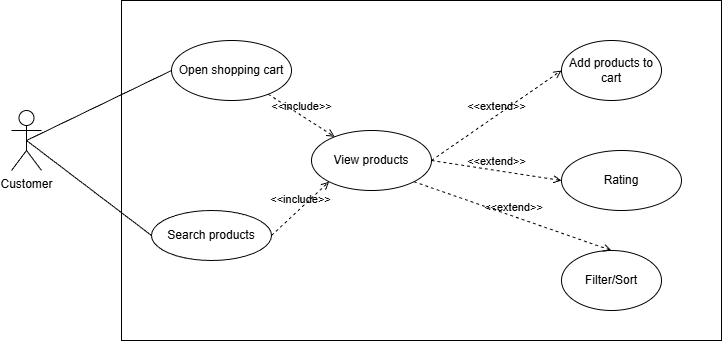
\includegraphics[width=\linewidth]{image/USE_CASE_ADD_PRODUCT.drawio.png}
    \label{fig:enter-label}
    \caption{Diagram use case của tính năng tìm kiếm và thêm sản phẩm vào giỏ hàng}
    \end{figure}
    \begin{longtable}{|>{\bfseries}p{4.5cm}|p{11cm}|} \hline 
Use case name: & Tìm kiếm và thêm sản phẩm vào giỏ hàng \\ \hline
Date created: & 11/10/2025 \\ \hline
Last updated date: & 30/11/2025 \\ \hline
Actor: & Customer \\ \hline
Description: & 
Customer có thể thực hiện mua hàng / thêm sản phẩm vào giỏ hàng / tìm kiếm sản phẩm  \\ \hline
Trigger: & 
Khi customer nhấn chọn biểu tượng " Tìm kiếm" hoặc khi customer chọn biểu tượng sản phẩm  \\ \hline
Pre-conditions: & 

Khách hàng đã đăng nhập vào hệ thống (hoặc có quyền truy cập như khách vãng lai nếu được phép). \newline
Hệ thống hoạt động bình thường, cho phép truy cập danh mục và thông tin sản phẩm. \newline
Dữ liệu về sản phẩm (tên, giá, mô tả, hình ảnh, tồn kho, v.v.) đã tồn tại trong cơ sở dữ liệu.\newline
Đối với các thao tác như thêm vào giỏ hàng (Add to shopping cart) hoặc chọn phương thức thanh toán (Choose payment method), khách hàng cần có giỏ hàng hợp lệ hoặc sản phẩm được chọn trước đó.\newline
Sản phẩm tồn tại. \\ \hline
Post-conditions: & 
Nếu quá trình thao tác thành công: \newline
Hệ thống hiển thị thông tin sản phẩm tương ứng (View product).\newline
Khách hàng có thể lọc sản phẩm (Filter) theo tiêu chí mong muốn.\newline
Khách hàng có thể thêm sản phẩm vào giỏ hàng (Add to shopping cart).\newline
Giỏ hàng được cập nhật và sẵn sàng cho quá trình thanh toán.\newline
Khách hàng có thể đánh giá sản phẩm (Rating) sau khi xem hoặc mua.
\\ \hline
Normal flow: &
1.Customer chọn biểu tượng tìm kiếm trên thanh tìm kiếm\newline
2.Hệ thống hiển thị sản phẩm gợi ý \newline
3. Customer có thể thêm sản phẩm vào giỏ hàng , xem thông tin sản phẩm và thao tác với sản phẩm hoặc giỏ hàng\newline
4.Sau khi trải nghiệm sản phẩm, customer có thể thực hiện đánh giá sản phẩm sau khi nhận hàng
\\ \hline
Alternative flow: &
2a.Nếu không tìm thấy được kết quả phù hợp trong bước tìm kiếm, hệ thống sẽ thông báo "Không tìm thấy sản phẩm", \newline
2b.Thay vì tìm kiếm cơ bản, customer có thể sử dụng filter để lọc sản phẩm\newline
2c.Customer mua trực tiếp không qua giỏ hàng
\\ \hline
Exception: &
Lỗi không tồn tại sản phẩm\newline
Lọc không trả về kết quả\newline
Tài khoản bị khóa nên không thực hiện được tác vụ\newline
Đánh giá không hợp lệ\newline
 \\ \hline
\caption{Đặc tả use case tính năng tìm kiếm/thêm sản phẩm vào giỏ hàng của người dùng }
\end{longtable}